\chapter{ARM M4}
The ARM M4 MCU is the heart of the stm32f407. ARM offers the IP of the
CORE-M4 to manufacturers and they can customize the IP as they see fit.
A very simple diagram of the used MCU is the following:\\

\begin{figure}[ht]
	\centering
	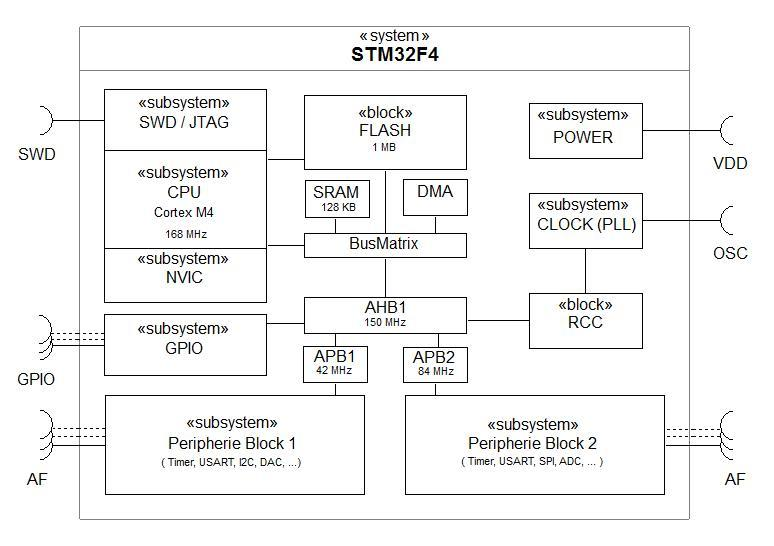
\includegraphics[width=400px,height=300px]{../img/stm32f4_prinzip.jpeg}
	\caption{Simple M4 Diagram}
	\label{m4_simple}
\end{figure}

The diagram doesn't show, which peripheral systems are connected to which
APBX-Bus\gls{apb}, but that can be seen in the datasheet. What it does show is, that
the GPIO-Pins, are connected to the AHB1-Bus\gls{ahb1}.\\
The reason for that is, that it's much faster then what is recommended
 for most the part of what a GPIO demands. The subsystems on the other hand aren't
 necessarily needed to react that fast.\\

For example the USART6, which is used in the project, is connected to APB2.
A much more precise representation of the STM32F4 is illustrated in the following diagram.\\

The AHB1 is the system bus and therefore should be really fast.
\includepdf[pages={18}]{../img/blockdia.pdf}
